%----------------------------------------------------------------------------------------
%	SLIDE 14.
%----------------------------------------------------------------------------------------
\begin{frame}
\frametitle{Parallelisation in physics}
\framesubtitle{Using Python}

\begin{exampleblock}{Prerequisites}
	\begin{itemize}
		\item E.g. the \texttt{threading}, \texttt{multiprocessing}, \texttt{joblib}, \texttt{subprocess} etc. packages mentioned in the previous section
		\item Multiple CPU cores available for ordering (e.g. this is $2$ in the case of Kooplex)
	\end{itemize}
\end{exampleblock}

\begin{figure}
	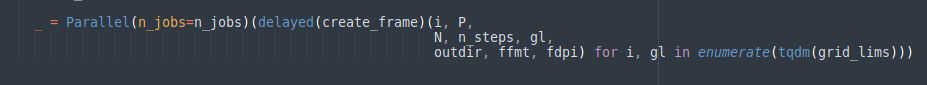
\includegraphics[width=\textwidth]{img/python-joblib.png}
\end{figure}

\begin{figure}
	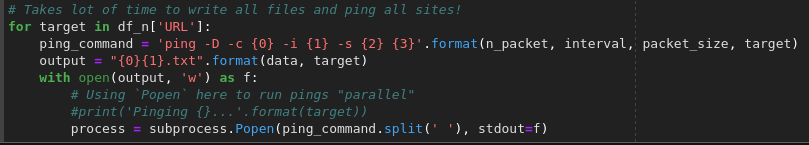
\includegraphics[width=\textwidth]{img/python-subprocess.png}
\end{figure}

\end{frame}